\chapter{ĐƠN HÌNH}
\section{Đơn hình chuẩn}
\indent Mỗi hình xuyến, mặt phẳng xạ ảnh ,bằng cách xác định các cạnh đối diện được chỉ ra bởi các vecto :
\begin{figure}[h]  
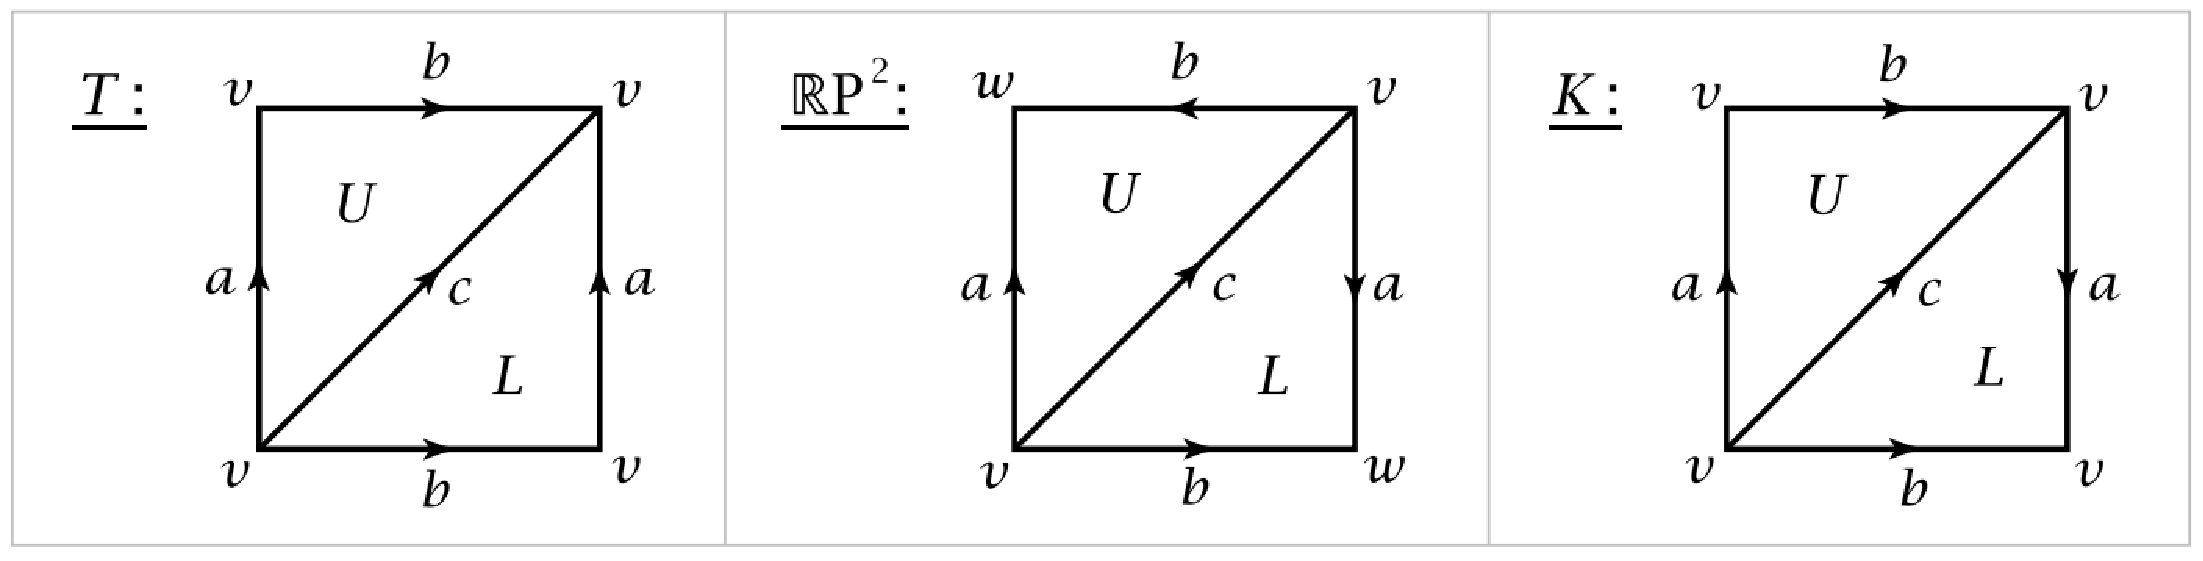
\includegraphics[width=\textwidth]{figures/chap1_1}
\caption[Cạnh đối diện vecto]{Cạnh đối diện vecto
\label{fig:chap1_1}}
\end{figure}

\indent Cắt một hình vuông theo một đường chéo sẽ tạo ra hai hình tam giác, vì vậy mỗi bề mặt này cũng có thể được dựng từ hai tam giác bằng cách xác định các cạnh của chúng theo từng cặp. Tương với một đa giác ,với bất kỳ số cạnh nào cũng có thể được cắt dọc đường chéo thành  hình tam giác. Như vậy, với đơn hình chuẩn \(n\) chiều \(\Delta_n\) , dễ dàng thấy \(\Delta_0\) là một điểm, \(\Delta_1\) là một đoạn thẳng, \(\Delta_2\) là một tam giác, \(\Delta_3\) là một tứ diện,...

\indent Đơn hình chuẩn tập lồi nhỏ nhất trong không gian Euclide \(R_m\) chứa \(n + 1\) điểm  \(v_0,\cdots,v_n\) không nằm trong một siêu phẳng có kích thước nhỏ hơn \(n\).
\newpage
\indent Ta có định nghĩa 1 \\
\indent Đơn hình chuẩn \(n\) chiều \(\Delta_n\) là một tập con của không gian \(R_{n+1}\) gồm các điểm \((t_0, t_1,\cdots, t_n) \in R^{n+1}\) thỏa mãn các điều kiện: \\
\indent a, \(t_i \geq 0\) , \(i = 0,1,\cdots,n\) \\
\indent b, \(\sum_{i=0}^{n}x_i=1\)

\section{Đơn hình kỳ dị}
\subsection[Định nghĩa 2]{Định nghĩa 2}
\indent Giả sử \(X\) là một không gian topo, đơn hình kỳ dị \(n\) chiều, \(n\geq0\), của không gian topo \(X\) là một ánh xạ liên tục từ đơn hình chuẩn \(\Delta_n\) vào không gian \(X\). \\
\indent Cho phép \(\Delta_n(X\)) là nhóm abel tự do với cơ sở là các đơn hình kỳ dị \(n\) chiều  mở \(e_\alpha^n\) của \(X\) . Các phần tử của \(\Delta_n(X)\), được gọi là dây chuyền kỳ dị \(n\) chiều , có thể được viết dưới dạng tổng chính thức hữu hạn \(\sum_{\alpha}n_\alpha$$e_\alpha^n$$\) với các đồng hiệu quả \(n_\alpha \in Z\) \\
\indent Tương tự, chúng ta có thể viết \(\sum_{\alpha}n_\alpha$$e_\alpha^n$$\)  trong đó \(\sigma_\alpha : \Delta_n\rightarrow$X$\) là bản đồ đặc trưng của \(e_\alpha^n\), với hình ảnh bao đóng của \(e_\alpha^n\) như mô tả ở trên. Như vậy tổng \(\sum_{\alpha}n_\alpha$$e_\alpha^n$$\) có thể được coi là một tập hợp hữu hạn. \\
\indent Như có thể thấy trong hình tiếp theo, ranh giới của đơn hình kỳ dị \(n\) chiều \([v_0,\cdots,v_n]\) bao gồm các đơn giản (n − 1) chiều khác nhau \([v_0,\cdots,\hat{v}_i,\cdots,v_n]\). Về mặt chuỗi, khi đó ranh giới của \([v_0,\cdots,v_n]\) là (n − 1) chuỗi được tạo bởi tổng các mặt \([v_0,\cdots, \hat{v}_i,\cdots,v_n]\). Tuy nhiên, để tốt hơn , thay vì chèn một số dấu hiệu, ta sẽ có  ranh giới của \([v_0,\cdots,v_n]\) là \(\sum_{i}(-1)^i[v_0,\cdots, \hat{v}_i,\cdots,v_n]\).\\
\begin{figure}[h]  
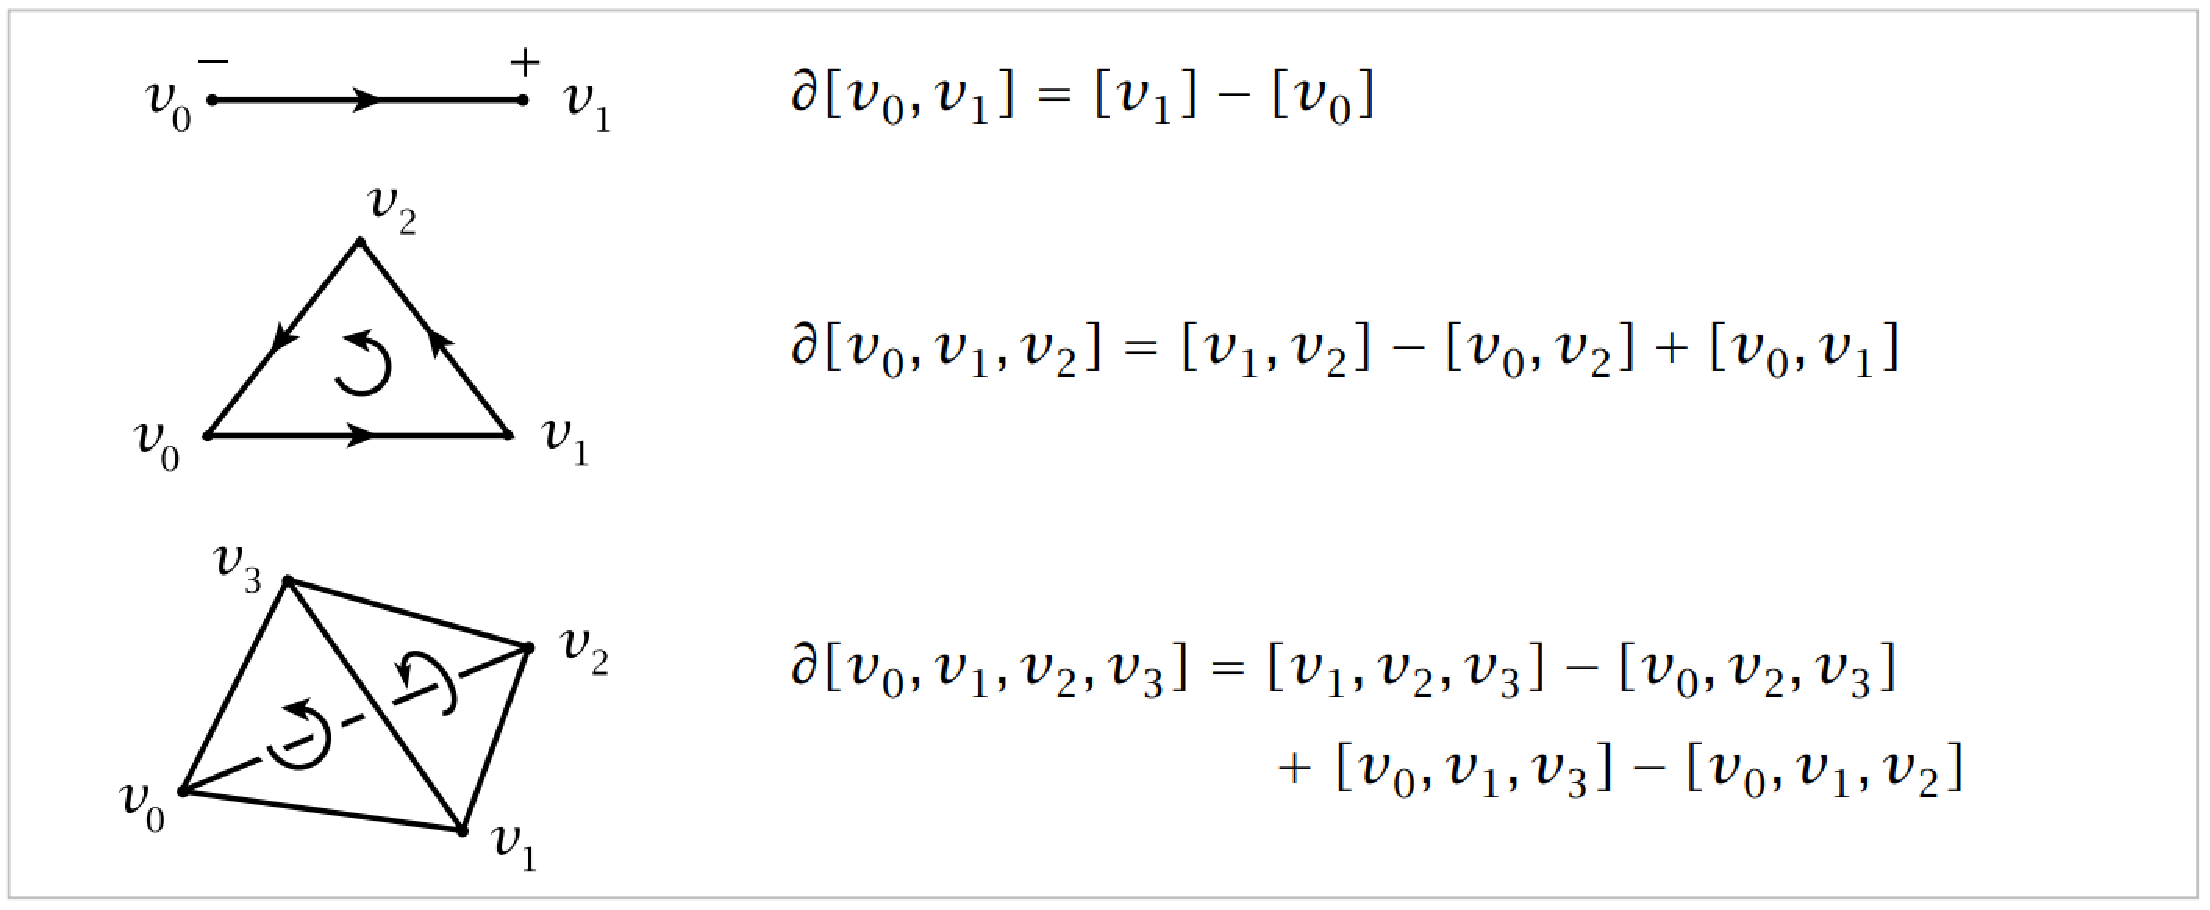
\includegraphics[width=0.9\textwidth]{figures/chap1_2}
\caption[Đơn hình kỳ dị n chiều]{Đơn hình kỳ dị n chiều
\label{fig:chap1_2}}
\end{figure}
\newpage
\indent Với hình học này, chúng ta xác định toán tử bờ \(\partial_n : \Delta_n(X)\rightarrow\Delta_{n-1} (X)\) bằng cách chỉ định các giá trị của nó trên các phần tử cơ sở: \[\partial_n(\sigma_\alpha) = \sum_{i}(-1)^i\sigma_\alpha|[v_0, \cdots,\hat{v}_i,\cdots,v_n]\].

\subsection[Bổ đề 1]{Bổ đề 1}
\indent Dãy phức  \(\Delta_n(X)\xrightarrow[]{\alpha_n}\Delta_{n-1}(X)\xrightarrow[]{\alpha_{n-1}}\Delta_{n-2}(X)\) là \(0\) \\
\indent Chứng minh: Ta có \[\partial_n(\sigma) = \sum_{i}(-1)^i\sigma|[v_0, \cdots,\hat{v}_i,\cdots,v_n]\] \\
\indent Và từ đây, \[\partial_{n-1}\partial_n(\sigma) = \sum_{j<i}(-1)^i(-1)^j\sigma|[v_0, \cdots,\hat{v}_i,\cdots,\hat{v}_j,\cdots,v_n]  + \sum_{j>i}(-1)^i(-1)^{j-1}\sigma|[v_0, \cdots,\hat{v}_i,\cdots,\hat{v}_j,\cdots,v_n] \] \\
\indent Tình huống đại số mà chúng ta có bây giờ là một dãy các đồng cấu của abelian các nhóm 
\[\cdots\rightarrow C_{n+1} \xrightarrow[]{\partial_{n+1}} C_{n} \xrightarrow[]{\partial_{n}} C_{n-1} \xrightarrow[]{\partial_{n-1}} \cdots \rightarrow C_1 \xrightarrow[]{\partial_{1}} C_0 \xrightarrow[]{\partial_{0}} 0 \]
với \(\partial_n\partial_{n+1} = 0\) với mỗi \(n\). Một chuỗi như vậy được gọi là một phức dây chuyền. \\
\indent Phương trình \(\partial_n\partial_{n+1} = 0\) tương đương với phép bao hàm Im \(\partial_{n+1} \subset\) Ker \(\partial_n\) , trong đó Im và Ker biểu thị hình ảnh và hạt nhân. \\
\indent Vì vậy, chúng ta có thể xác định nhóm tương đồng thứ \(n\) phức hợp dây chuyền là nhóm thương \(H_n =\) Ker \(\partial_n / \) Im \(\partial_{n+1}\) . \\
\indent Các phần tử của Ker \(\partial_n\) được gọi là chu trình và các phần tử của Im \(\partial_{n+1}\) được gọi là biên.  \\
\indent Các phần tử của \(H_n\) của Im \(\partial_{n+1}\) , được gọi là các lớp tương đồng. \\
\indent Trở lại trường hợp \(C_n = \Delta_n(X)\), nhóm tương đồng Ker \(\partial_n/\) Im \(\partial_{n+1}\) sẽ được ký hiệu là \(H_n\Delta(X)\) và được gọi là nhóm đồng đẳng đơn giản thứ \(n\) của \(X\) . 
\newpage

\begin{figure}[h]
	\centering
	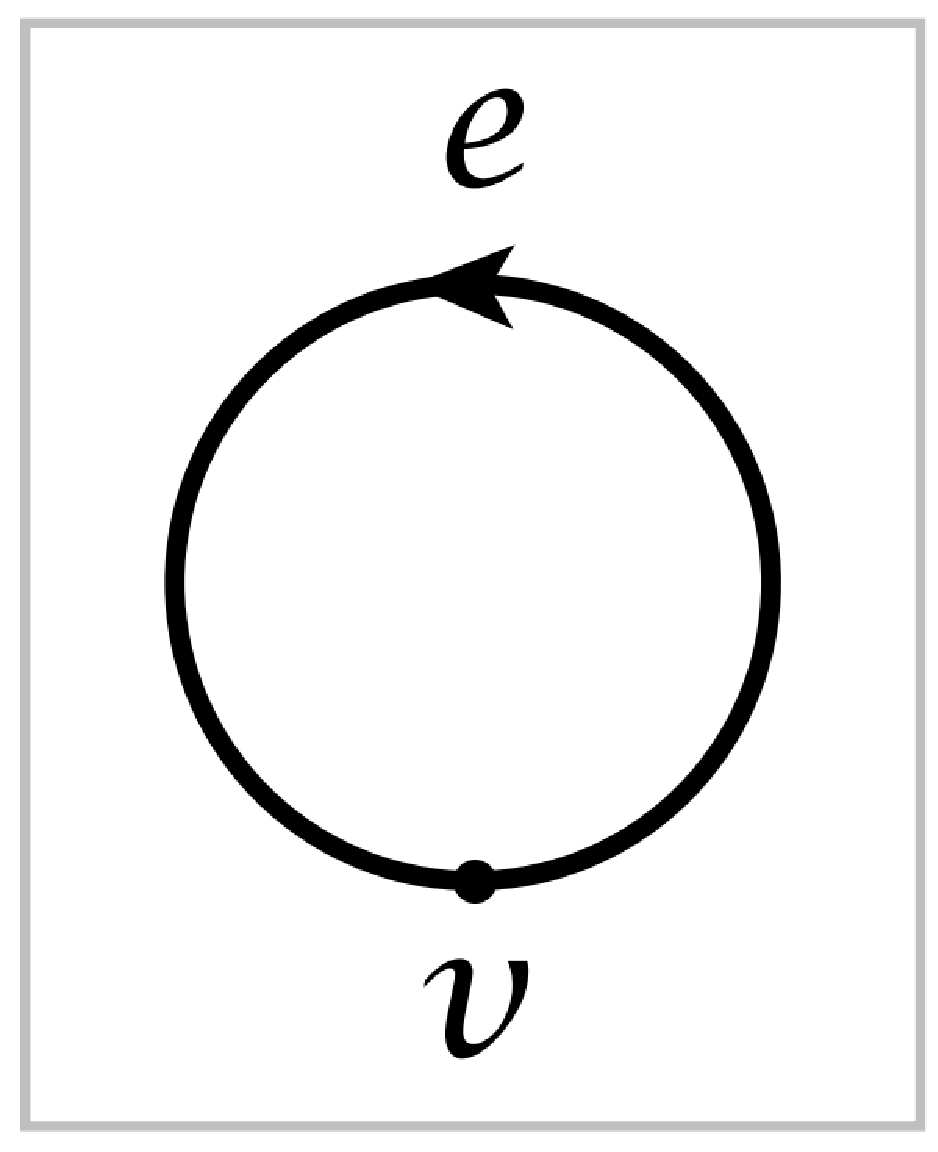
\includegraphics[scale=0.2]{figures/chap1_3}
	\caption[Ví dụ bổ đề 1]{Ví dụ bổ đề 1
	\label{fig:chap1_3}}
\end{figure}

\textbf{Ví dụ 1.} (Hình 1.2.2) \\
\indent \(X = S^1\), với một đỉnh \(v\) và một cạnh \(e\). Khi đó \(\Delta_0 (S^1)\) và \(\Delta_1 (S^1)\) đều là $\mathds{Z}$ và là ánh xạ biên \(\partial_1\) bằng 0 vì \(\partial_e\) = v −v . Các nhóm \(\Delta_n(S1)\) bằng 0 với \(n \geq 2\) vì không có đơn giản nào trong các nhóm này kích thước. Kể từ đây: \[H_n^{\Delta}(S^1) \approx \begin{cases}
\mathds{Z} & \text{for $n$ = 0,1}\\
0 & \text{for $n$} \geq 2
\end{cases} 
\] 

\textbf{Ví dụ 2.} (Hình 1.2.2) \\
\indent \(X = T\) , hình xuyến có cấu trúc phức tạp \(\Delta\) , có một đỉnh, ba cạnh \(a\), \(b\) và \(c\) và hai 2 mặt phẳng \(U\) và \(L\). Với \(\partial_1\) = 0 nên \(H_0^{\Delta} (T) \approx \mathds{Z}\) . \\
Vì \(\partial_2U\) = a + b − c = \(\partial_2L\) và \{a, b, a + b − c\} là một cơ sở cho \(\Delta_1(T)\), suy ra \\
\(H_1\Delta(T) \approx  \mathds{Z} \oplus \mathds{Z}\) với cơ sở là các lớp tương đồng \([a]\) và \([B]\). \\
Vì không tồn tại 3 số đơn giản nên \(H_2^{\Delta}(T)\) bằng Ker \(\partial_2\) , là vô hạn tuần hoàn được tạo bởi U − L vì \(\partial(pU + qL)\) = \((p + q)(a + b\) − c) = 0 chỉ khi \(p\) = −\(q\). Như vậy:
\[H_n^{\Delta}(T) \approx \begin{cases}
	\mathds{Z} \oplus \mathds{Z} & \text{for $n$ = 1}\\
	\mathds{Z} & \text{for $n$ = 0,2} \\
	0 & \text{for $n$} \geq 3
\end{cases} 
\] \\